\documentclass[runningheads]{llncs}
\usepackage[T1]{fontenc}
\usepackage[utf8]{inputenc}
\usepackage{graphicx}
\usepackage{booktabs}
\usepackage{amsmath,amssymb}
\usepackage{url}
\usepackage{color}
\renewcommand\UrlFont{\color{blue}\rmfamily}
\setlength{\textfloatsep}{7pt plus 2pt minus 2pt}
\setlength{\floatsep}{7pt plus 2pt minus 2pt}

\begin{document}
\title{From Observation to Action: When Does Hypothesis Testing Help Agents Discover Hidden Rules?}
\titlerunning{Hypothesis Testing for Hidden-Rule Discovery}
\author{Arti}
\authorrunning{Arti}
\institute{IILM University, Greater Noida, India}
\maketitle

\begin{abstract}
@@ABSTRACT@@
\keywords{Rule discovery \and Hypothesis testing \and Posterior sampling \and Compositional generalization \and Learned agents.}
\end{abstract}

\section{Introduction}
Agents deployed in new environments rarely get the rules explained; they must infer them from the consequences of their own actions: which key opens which door, which lever order unlocks a vault. This is close in spirit to measuring skill-acquisition efficiency rather than skill on a fixed distribution~\cite{chollet2019}. Three mechanisms are commonly proposed: explicit \emph{hypothesis testing}~\cite{klahr1988,gopnik1997,tenenbaum2011}, Bayesian \emph{posterior sampling}~\cite{strens2000,osband2013}, and \emph{learned} policies whose recurrent state implements adaptation~\cite{duan2016,wang2016}. We compare them in controlled, fully inspectable benchmarks and ask four questions. \textbf{Q1:} does explicit hypothesis testing beat reactive, Bayesian and learned agents, and where? \textbf{Q2:} which ingredients (reward form, information bonus, memory, revision, structural assumptions) account for the differences? \textbf{Q3:} must the testable-action vocabulary be supplied, or can a learned agent find it from generic skills? \textbf{Q4:} do the findings replicate in a second, structurally different environment family?

This is an independent benchmark study; it does not reproduce ARC-AGI-3 or any external benchmark, uses no language models, and makes no claim about general intelligence. \textbf{Contributions.} (1) A procedural grid-world benchmark with six generalization regimes and rule-type and assumption-violation variants, plus a second family (a combination vault). (2) A hypothesis-driven agent, a posterior-sampling agent, and learned agents over testable macro-actions, over generic skills and over primitives, with three training seeds for the learned agents. (3) A factorial ablation separating reward form from the information bonus. (4) A proposition predicting the failed-test cost of evidence elimination, confirmed in both families. (5) An account of what fails: learned agents extrapolate poorly, and the agent's structural assumptions can be catastrophic when false.

\section{Related Work}
Procedural benchmarks (Procgen, BabyAI, Minigrid~\cite{cobbe2020,chevalier2019,chevalier2023}) expose train--test gaps surveyed in~\cite{kirk2023}; we make rule \emph{bindings} the object of discovery. Compositional generalization is studied mainly in language~\cite{lake2018,keysers2020}. Exploration with information gain~\cite{bellemare2016,pathak2017,houthooft2016} and active learning~\cite{settles2009} motivate our utility, computed here over a symbolic hypothesis space. Posterior sampling~\cite{thompson1933,strens2000,osband2013} and Bayesian RL~\cite{ghavamzadeh2015} give our Bayesian baseline; recurrent meta-RL~\cite{duan2016,wang2016,finn2017,zintgraf2020} and temporal abstraction~\cite{sutton1999} give our learned baselines. We follow guidance on seeds and uncertainty in RL evaluation~\cite{henderson2018,colas2018,agarwal2021}.

\section{Benchmarks}
\textbf{Grid family.} Grids ($8$--$14$ cells wide) contain walls, keys, doors, switches, chasms, movable blocks, traps and a target; actions are UP, DOWN, LEFT, RIGHT, INTERACT, PUSH, WAIT; observations are fully observable and never expose the hidden rules. Gate rules are composed procedurally: \emph{key--door} (one key carried at a time; key color $k$ opens door $\phi(k)$), \emph{switch--bridge}, \emph{push-block} (two pushes), and, for rule-type discovery, \emph{switch--door}. Bindings are redrawn per environment. Each gate's key or switch lies in an earlier zone, so instances are solvable by construction (verified by a solver). Difficulty 1--5 adds gates, distractor keys/switches and traps; episodes last at most 200 steps. Table~\ref{tab:regimes} lists the generalization regimes; train and test use disjoint seeds, and regime D uses disjoint color symbols with the relation (key color equals door color) preserved.

\textbf{Combination vault.} A hidden injective sequence of $k$ levers (of $L$) must be pressed in order; a correct press advances, a wrong press resets progress (feedback: advance, reset, open). There is no navigation, the hypothesis space is sequences rather than pairings, and success requires remembering which levers failed at which position. Learned agents train on $L\in\{4,5\},k\in\{2,3\}$ and are tested also on $L\in\{6,7\},k\in\{4,5\}$ (150 steps).

@@TAB_REGIMES@@
@@TAB_ENV@@

\section{Agents}
All non-random agents avoid traps and know the action semantics; what they must discover are the bindings (and, in one experiment, rule types).

\textbf{Reactive} uses BFS heuristics on the current observation plus one lose-shift bit; it records which pairs it tried in no form. \textbf{Hypothesis-driven (ours)} keeps hypotheses (key color, door color), (switch, chasm) and ``blocks are pushable'' with confidences: a correct prediction adds $\alpha=0.6$ and confirms the hypothesis, a wrong one subtracts $\beta=0.6$ and rejects it after two contradictions; probabilities are normalized over non-rejected candidates with mutual exclusion. State is recomputed from episodic memory entries, so memory capacity controls what is remembered. Decisions are over macro-actions (go to target, pick or swap a key, test the held key on a door, toggle a switch, push a block) scored by
\begin{equation}
U(a)=R(a)+\lambda\,IG(a)-\mu\,c(a),\quad R=V\!\cdot\!p,\ \ IG=\textstyle\sum H_b(p),\ \ c=\text{path length},
\end{equation}
with $V=3$ per gate (10 for the target), $\lambda=0.5$, $\mu=0.05$. \textbf{PSRL}~\cite{strens2000,osband2013} uses the same evidence but keeps a sticky sampled binding consistent with all outcomes and acts as if it were true; it resamples when the sample offers no progress. In the vault the hypothesis agent is the explicit set of all consistent codes, pressing the lever with the highest posterior probability.

\textbf{Learned agents} are trained with PPO~\cite{schulman2017} in JAX~\cite{jax2018} (feedforward and GRU~\cite{cho2014}). \emph{Macro} agents choose among exactly the macro-actions above, with features limited to macro type, colors involved and path cost, plus the last macro and its outcome: no belief features. \emph{Generic} agents choose among generic skills only (go to a key, switch, door, block or target; INTERACT; PUSH), so the testing structure must be learned. \emph{Primitive} PPO acts on a CNN encoding of the grid with potential-based shaping~\cite{ng1999}. Macro and generic agents have three (macro) or two (generic) independent training seeds per distribution and one model per regime, trained only on that regime's training distribution. Vault agents are PPO feedforward and GRU with three seeds.

@@TAB_AGENTS@@

\section{Protocol and a Simple Analysis}
Every cell uses @@NSEEDS@@ evaluation seeds $\times$ @@NENV@@ fresh environments (seed is the unit of analysis; evaluation seed $s$ uses trained model $s \bmod m$); primitive PPO uses fewer, as inference is slower. We report means with 95\% bootstrap intervals~\cite{efron1993}, Welch's $t$~\cite{welch1947} with Holm correction~\cite{holm1979} over all @@NTESTS@@ tests, and Cohen's $d$~\cite{cohen1988}.

\begin{proposition}
Let one door have $n$ equally likely candidate keys, exactly one correct. (i) Elimination (never retest a failed key) has $\mathbb{E}[\text{failed tests}]=(n-1)/2$. (ii) A stateless lose-shift strategy (uniform start, then a uniformly random key other than the one in hand) has $(n-1)^2/n$; the excess $(n-1)(n-2)/(2n)$ is $0$ for $n=2$ and grows linearly. In the vault, elimination gives $\sum_{p=0}^{k-1}(L-p-1)/2$ resets.
\end{proposition}
\begin{proof}[sketch]
(i) The test order is a uniform permutation, so failures before success are uniform on $\{0,\dots,n-1\}$. (ii) The first test fails with probability $(n-1)/n$; later attempts succeed with probability $1/(n-1)$ each, giving $n-2$ further failures on average, so $\frac{n-1}{n}(1+(n-2))=(n-1)^2/n$. The vault sum applies (i) at each position, where $L-p$ levers remain.
\end{proof}

\section{Results}
@@RES_MAIN@@
@@TAB_MAIN@@
\begin{figure}[t]
\centering
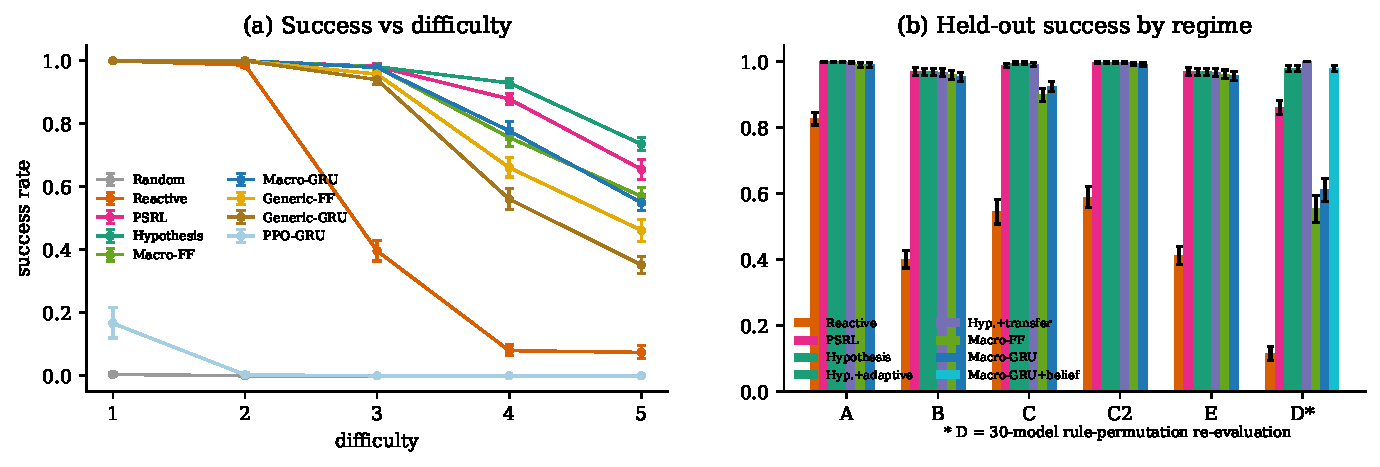
\includegraphics[width=\linewidth]{figures/fig15_main.pdf}
\caption{(a) Success versus difficulty; (b) held-out success per generalization regime (A--E, C2). Bars are 95\% bootstrap intervals over seeds.}\label{fig:main}
\end{figure}
@@RES_GEN@@
@@RES_ISO@@
\begin{figure}[t]
\centering
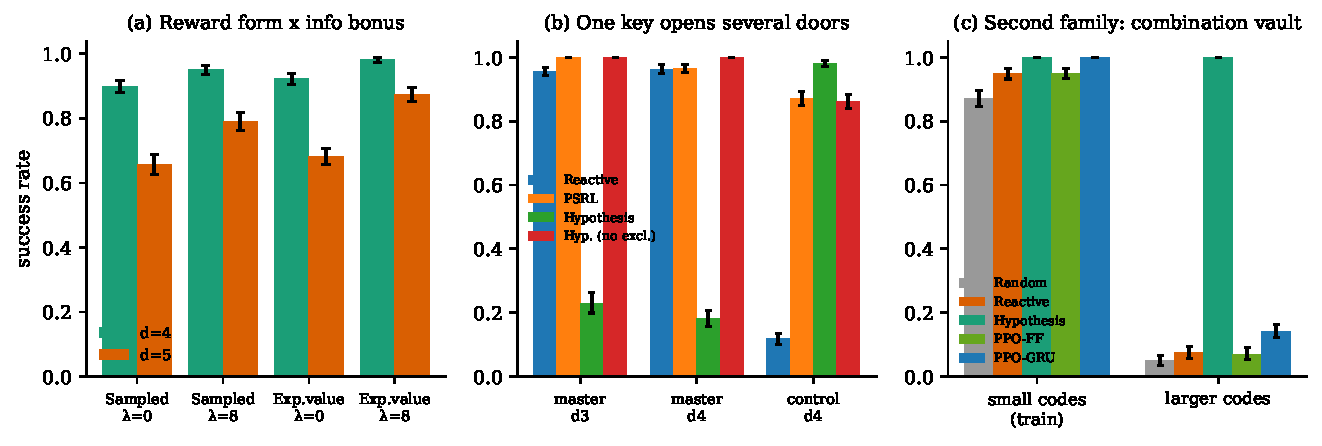
\includegraphics[width=\linewidth]{figures/fig16_ablate.pdf}
\caption{(a) Factorial ablation (difficulties 4 and 5); (b) master-key environments, where one key opens several doors, and an exclusive control; (c) the combination vault: small codes (training distribution) and larger codes.}\label{fig:ablate}
\end{figure}
\begin{figure}[t]
\centering
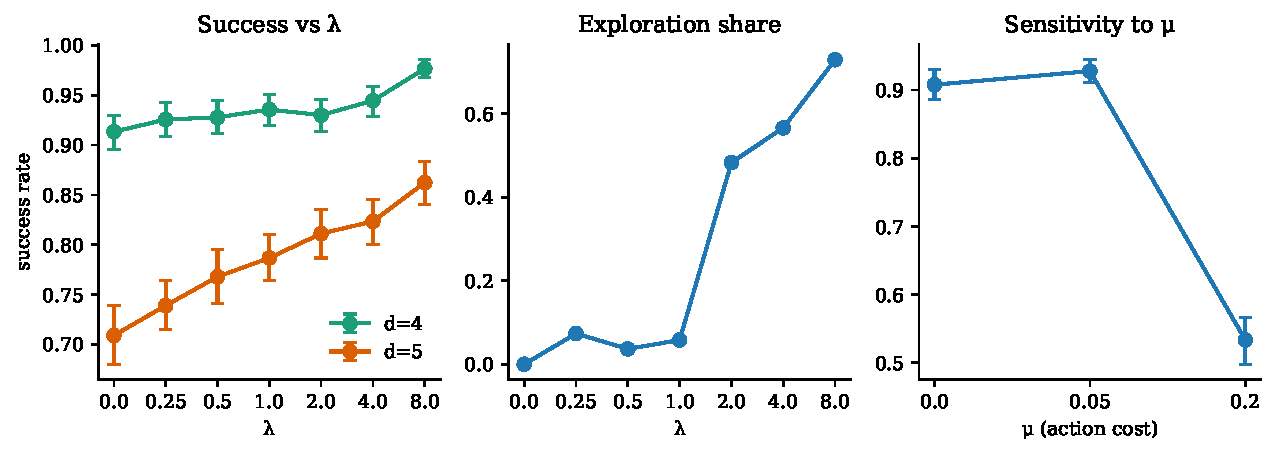
\includegraphics[width=.92\linewidth]{figures/fig10_explore_exploit.pdf}
\caption{Information-gain weight $\lambda$ (difficulties 4 and 5), exploration share, and action-cost weight $\mu$.}\label{fig:lambda}
\end{figure}
@@TAB_ABL@@
@@RES_VOCAB@@
@@TAB_SEEDS@@
@@RES_VAULT@@
@@RES_MISC@@
\begin{figure}[t]
\centering
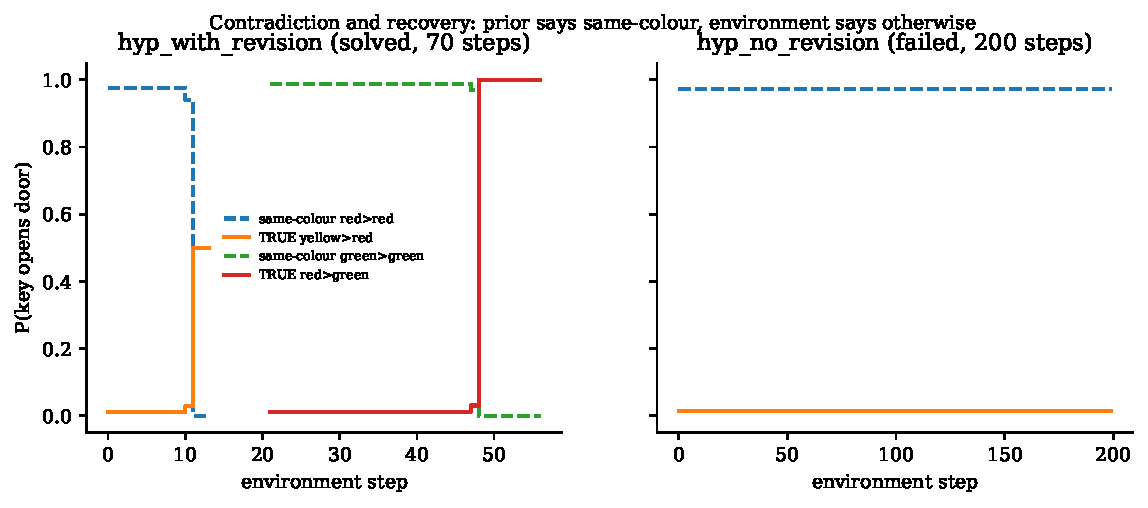
\includegraphics[width=.85\linewidth]{figures/fig8_contradiction_recovery.pdf}
\caption{Hypothesis probabilities in one held-out environment where a learned same-color prior is wrong: with revision the true bindings are found, without it the agent persists.}\label{fig:rec}
\end{figure}

\section{Discussion and Limitations}
@@DISCUSS@@

\section{Conclusion}
@@CONCL@@

\section{Reproducibility}
Code, tests, configuration and the one-command pipeline are in the supplementary archive; every number is read from \texttt{data/results/*.csv} by \texttt{paper/build\_paper.py}, and secondary tables (ablations, scaling, all significance tests) are in \texttt{paper/tables/}. Everything runs on one CPU core with 3~GB RAM. We found and fixed several bugs in our own agents and baselines before reporting (refuted-hypothesis retest loops, a posterior-sampling sample that assigned an unreachable key, two defects in the shaping signal of primitive PPO, and an evaluation stage that overwrote results); no pre-fix results appear here.

\bibliographystyle{splncs04}
\bibliography{references}
\end{document}
